\subsection{Schwerpunktverteilung mit Gleitkommazahlen}
\begin{table}[h!]
    \hspace{-0.5cm}
    \begin{tabular}{ | l | c | c | c | c |}
        \hline
        Konfiguration & Beste & Unter 60 kB & Unter 28 kB & Unter 14 kB \\\hline
        Ensemble-Methode & Boosting & Boosting & RandomForest & Bagging  \\\hline
        Maximalhöhe & 20 & 19 & 10 & 7 \\\hline
        Waldgröße & 10 & 6 & 4 & 3 \\\hline
        min\_samples\_leaf & 8 & 8 & 2 & 8 \\\hline
        Programmgröße in Bytes & 83304 & 43678 & 20188 & 6656 \\\hline
        Genauigkeit Testmenge von Klisch & 94,8\% & 94.8\% & 89,6\% & 87,5\% \\\hline
        Genauigkeit Gestentestmenge & 97,0\% & 96,1\% & 95,6\% & 94,1\% \\\hline
        Genauigkeit Nullgestentestmenge & 92,2\% & 91,1\% & 88,8\% & 89,9\% \\\hline
    \end{tabular}
    \caption{Beste Konfigurationen der Schwerpunktverteilung mit Gleitkommazahlen.}
    \label{tab:schwerpunktverteilung_float}
\end{table}
\begin{figure}[h!]
    \centering
    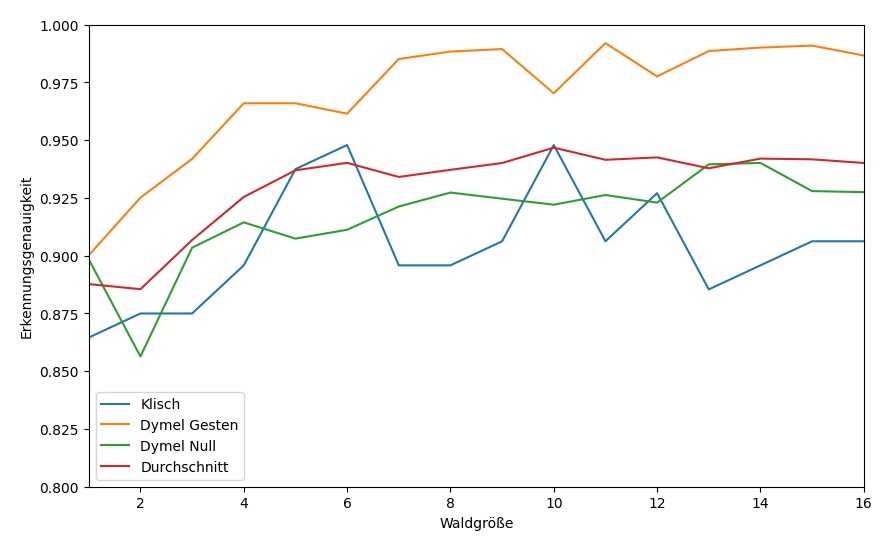
\includegraphics[width=\linewidth]{images/cocd_float_acc_per_size.png}
    \caption{Die beste summierte Erkennungsgenauigkeit pro Waldgröße der Schwerpunktverteilung mit Gleitkommazahlen.}
    \label{fig:cocd_float_per_forest_size}
\end{figure}
Die Featuremenge Schwerpunktverteilung mit Gleitkommazahlen folgt der Definition aus Sektion \ref{sec:schwerpunktverteilung} und beinhaltet insgesamt 10 Einträge, wobei jeweils 2 Einträge die X und Y
Koordinate des Schwerpunktes darstellen in insgesamt 5 Zeitfenstern.
\newline
\newline
Die beste Konfiguration wurde mit der Ensemble-Methode Boosting erzielt (siehe Tabelle \ref{tab:schwerpunktverteilung_float}). Mit einer Erkennungsgenauigkeit von 94,8\% auf der Testmenge von Klisch
ist dieser Ansatz nur 5,2\% schlechter als das neuronale Netz von Giese \cite{gieseThesis}. Es ist anzumerken, dass mit einer kleineren Trainingsmenge ohne die Gestentrainingsmenge und Nullgestentrainingsmenge eine Lösung
gefunden wurde, die 97,9\% erzielte und damit nur 2,1\% schlechter ist. Außerdem werden 97\% der Gestentestmenge und 92,2\% der Nullgestentestmenge korrekt klassifiziert.
\newline
\newline
Im Vergleich zu der Helligkeitsverteilung und Motion History ist die Erkennungsgenauigkeit dieses Ansatzes signifikant besser, sogar wenn nur 6656 Byte Programmspeicher verwendet werden. Wird die beste Konfiguration mit
der \textit{Unter 14 kB} verglichen, nimmt die Gesamterkennungsganuigkeit nur um 4,17\% ab bei der Reduktion der Programmgröße von 92\%. Dies verspricht, dass mit zunehmender Waldgröße der die Erkennungsgenauigkeit steigt.
Abbildung \ref{fig:cocd_float_per_forest_size} zeigt, dass dies zwar der Fall ist, aber schon ab einer Waldgröße von 6 ist die Durchschnittliche Erkennungsgenauigkeit keinen signifikanten Zuwachs mehr verzeichnet.
Dementsprechend ist der Unterschied der Gesamterkennungsgenauigkeit der besten Konfiguraiton und \textit{Unter 60 kB} mit 0,7\% nicht groß, wodurch sich dieses Feature gut für kleine eingebettete Systeme mit
wenig Programmspeicher eignet.